\documentclass{beamer}
% Copyright 2015 by Do Phan Thuan

% Loại mẫu slice
%\usetheme{AnnArbor}
%\usetheme{Antibes}
\usetheme{Boadilla}
%\usetheme{CambridgeUS}
%\usetheme{Hannover}

% Ký tự tiếng Việt
\usepackage[utf8]{vietnam}
\usepackage[utf8]{inputenc}
% Công thức toán
\usepackage{amsmath,amsthm,amssymb,epsfig}
% Chèn ảnh
\usepackage{graphicx}
% Chèn đường dẫn 
\usepackage{url}

% Vẽ đồ thị
\usepackage{pgfplots}

% Insert code
\usepackage{listings}
\lstset{language=C++,
   %keywords={break,case,catch,continue,else,elseif,end,for,function,
   %   global,if,otherwise,persistent,return,switch,try,while},
   basicstyle=\ttfamily,
   keywordstyle=\color{blue},
   commentstyle=\color{red},
   stringstyle=\color{dkgreen},
   frame=lrtb,
   %frame=5 pt,
   numbers=left,
   numberstyle=\tiny\color{gray},
   stepnumber=1,
   numbersep=10pt,
   backgroundcolor=\color{white},
   tabsize=4,
   showspaces=false,
   showstringspaces=false}
% Tô mầu cho bảng
\usepackage{colortbl}


\usepackage{color}

\definecolor{dkgreen}{rgb}{0,0.6,0}
\definecolor{gray}{rgb}{0.5,0.5,0.5}
\definecolor{mauve}{rgb}{0.58,0,0.82}
  
\definecolor{Xanh}{rgb}{0,0.5,1}
\definecolor{Do}{rgb}{1,0.25,0}
\definecolor{Vang}{rgb}{1,1,0}
\definecolor{Datroi}{rgb}{0,0,1}
% Vẽ hình
\usepackage{tikz}
\usetikzlibrary{arrows,shapes}
% Vẽ mạch điện
\usepackage[siunitx,european resistors]{circuitikz}

% multirow
\usepackage{multirow}

\usepackage{pbox}

% Tô mầu cho bảng
\usepackage{colortbl}
\definecolor{Xanh}{rgb}{0,0.5,1}
\definecolor{Do}{rgb}{1,0.25,0}
\definecolor{Vang}{rgb}{1,1,0}
\definecolor{Datroi}{rgb}{0,0,1}

% Một vài ký hiệu thường dùng
\def\R{{\mathbb R}}
\def\N{{\mathbb N}}
\def\X{{\mathcal X}}
\def\Y{{\mathcal Y}}
\def\F{{\mathcal F}}
\def\P{{\mathcal P}}
\def\E{{\mathbb E}}
\def\I{{\mathbb I}}
\def\sign{{\rm sign}}

% Xác định khoảng dãn trong bảng
\renewcommand\arraystretch{1.2}

% a few macros
\newcommand{\bi}{\begin{itemize}}
\newcommand{\ei}{\end{itemize}}
\newcommand{\ig}{\includegraphics}
\newcommand{\subt}[1]{{\footnotesize \color{subtitle} {#1}}}

% named colors
\definecolor{offwhite}{RGB}{249,242,215}
\definecolor{foreground}{RGB}{255,255,255}
\definecolor{background}{RGB}{24,24,24}
\definecolor{title}{RGB}{107,174,214}
\definecolor{gray}{RGB}{155,155,155}
\definecolor{subtitle}{RGB}{102,255,204}
\definecolor{hilight}{RGB}{22,155,104}
\definecolor{vhilight}{RGB}{255,111,207}
\definecolor{lolight}{RGB}{155,155,155}
%\definecolor{green}{RGB}{125,250,125}

% Minted
%\usepackage{minted}
%\usemintedstyle{monokai}
%\newminted{cpp}{fontsize=\footnotesize}

% Graph styles
\tikzstyle{vertex}=[circle,fill=black!50,minimum size=15pt,inner sep=0pt, font=\small]
\tikzstyle{selected vertex} = [vertex, fill=red!24]
\tikzstyle{edge} = [draw,thick,-]
\tikzstyle{dedge} = [draw,thick,->]
\tikzstyle{weight} = [font=\scriptsize,pos=0.5]
\tikzstyle{selected edge} = [draw,line width=2pt,-,red!50]
\tikzstyle{ignored edge} = [draw,line width=5pt,-,black!20]

%gets rid of bottom navigation bars
\setbeamertemplate{footline}[frame number]{}

%gets rid of bottom navigation symbols
%\setbeamertemplate{navigation symbols}{}

%gets rid of footer
%will override 'frame number' instruction above
%comment out to revert to previous/default definitions
%\setbeamertemplate{footline}{}

% Tác giả, Tiêu đề, vân vân
\title[]{{\bf \large HyperLogLog in Practice: Algorithmic Engineering of a
State of The Art Cardinality Estimation Algorithm } \\
}
\author[]{
Nguyễn Tuấn Đạt \\% \inst{1} 
Đặng Quang Trung% \inst{1} 
}

\institute[]{
%\inst{1}% 

}

\logo{
\includegraphics[scale=0.05]{hust.jpg} \vspace{220pt}}

\begin{document}

\begin{frame}
\titlepage
\end{frame}

\begin{frame}{Nội dung}
\tableofcontents
\end{frame}
\section{Giới thiệu}

\begin{frame}{Giới thiệu bài toán Cardinality estimation}
\subsection{Cardinality estimation}
Là bài toán xác định số lượng phần tử khác nhau trong một data stream. 

Các yêu cầu :
\begin{itemize}
\item Accuracy(Độ chính xác)
\item Memory efficiency( Hiệu quả sử dụng bộ nhớ)
\item Estimate large cardinalities(Ước lượng một tập rộng)
\item Practicality.(Tính thực tế)
\end{itemize}

\end{frame}
\begin{frame}{Thuật toán HyperLogLog}
\subsection{Thuật toán HyperLogLog}
Thuật toán sử dụng yếu tố ngẫu nhiển để xấp xỉ lực lượng của một multiset.\\
Yếu tố ngẫu nhiên được thực thi bằng cách sử dụng hàm băm H cho mọi biến của tập.\\
Thuật toán sẽ đếm số lượng số 0 ở đâù của giá trị băm $ 0^{\varrho-1} 1 $ có ước lượng cho tập đó có thể là $ 2^\varrho$ 
\end{frame}
\begin{frame}
\begin{figure}[h]
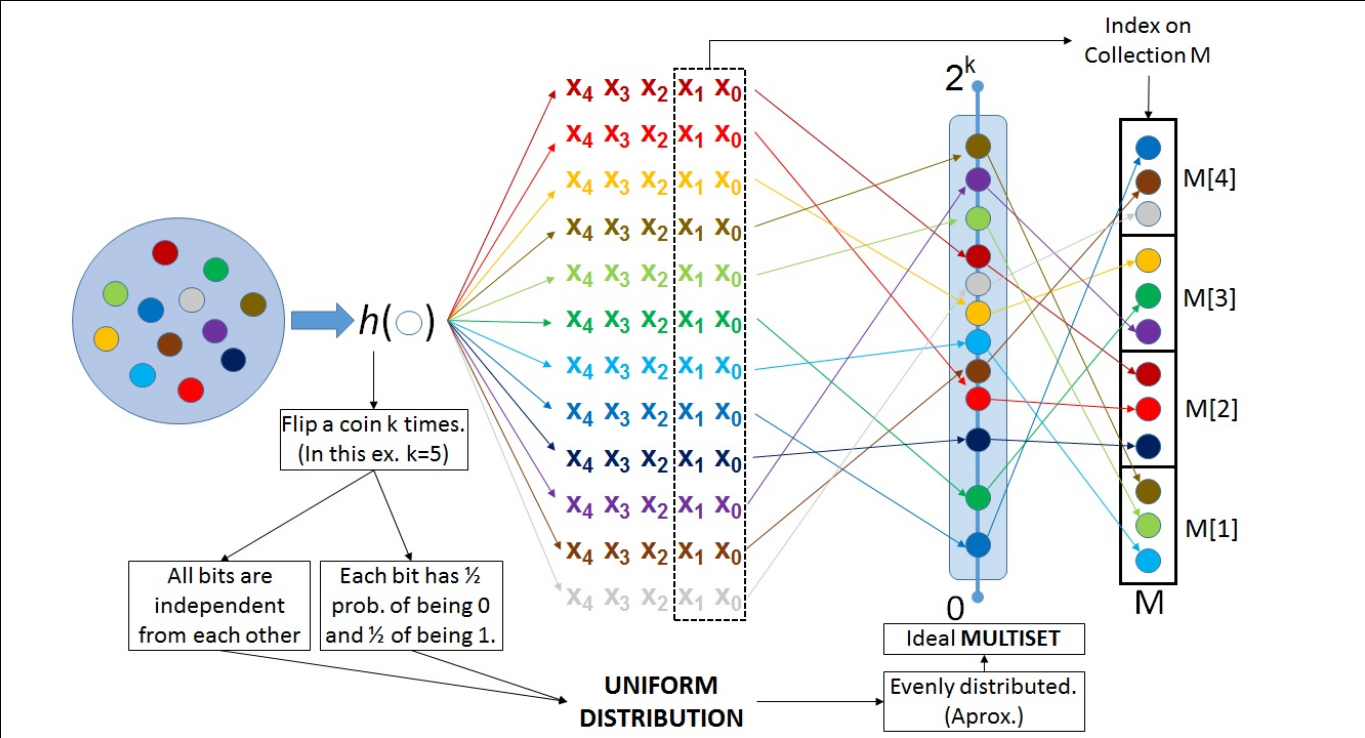
\includegraphics[scale=0.2]{HLL.png}
\caption Thuật toán Hyper Log Log
\end{figure}
\end{frame}
\begin{frame}
\begin{figure}[H]
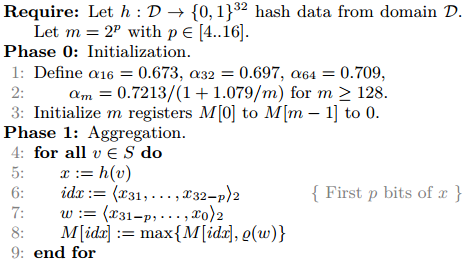
\includegraphics[scale=0.3]{HLL1.png}

\end{figure}
\end{frame}
\begin{frame}
\begin{figure}[H]
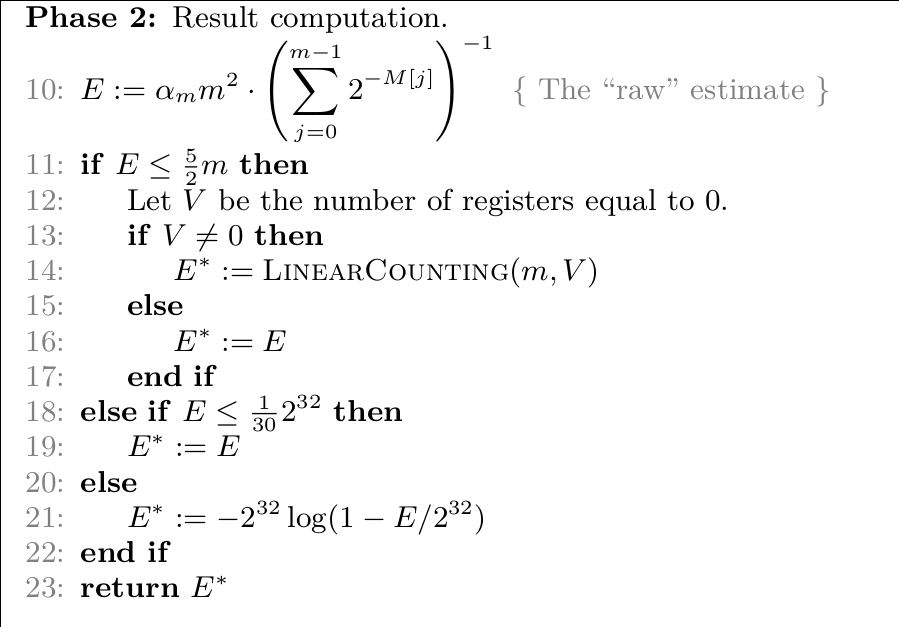
\includegraphics[scale=0.3]{HLL2.png}
\end{figure}
\end{frame}

\begin{frame}{Giải thích chi tiết}
\begin{enumerate}
\item Initialization of registers
\item Small range corrections
\item Large range corrections.
\end{enumerate}
\end{frame}
\section{Các cải tiến cho HyperLogLog }
\begin{frame}{Các cải tiến cho HyperLogLog}

\end{frame}
\begin{frame}{Sử dụng hàm băm 64 bit}
\subsection{Sử dụng hàm băm 64bit}
\begin{itemize}
\item[•] Hàm băm L bits có thể có $2^L$ giá trị phân biệt. Nếu lực lượng của tập n có $2^L$ biểu diễn thì xung đột hàm băm có khả năng nhiều xảy ra $\rightarrow$ ước lượng chính xác là không thể.
\item[•] Yêu cầu bộ nhớ $\lceil log_2(L + 1 - p) \rceil .2^p$ bits
\begin{itemize}
\item L bits hàm băm, độ chính xác p.
\end{itemize}
\item[•] Sử dụng 64 bits yêu cầu bộ nhớ $6.2^p$
\begin{itemize}
\item không cần quan tâm xung đột hàm băm \\
(lực lượng tập $2^64 \approx 1.8\cdot 10^{19}$ )
\item Large range correction là không cần thiết 
\end{itemize}
\end{itemize}
\end{frame}


\begin{frame}{Ước lượng cho tập lực lượng nhỏ(Estimating Small Cardinalities)}
\subsection{Estimating Small Cardinalities}
\begin{itemize}
\item[•] Ước lượng $HLL_{ORIG}$ gặp lỗi lớn đối với tập có lực lượng nhỏ
\begin{itemize}
\item[•] Nếu n = 0 thuật toán luôn trả về 0.7m 
\end{itemize}
\item[•] Để đạt được ước lượng tốt cho tập lực lượng nhỏ
\begin{itemize}
\item $HLL_{ORIG}$ sử dụng LINEARCOUNTING nếu $E < \frac{5}{2}m$ ngược lại dùng ước lượng thô. 
\end{itemize}
\item[•] Các lỗi của ước lượng thô là vì độ lệch
\begin{itemize}
\item Chúng ta có thể hiệu chỉnh độ lệch
\item Chúng ta hi vọng sẽ đạt được ước lượng tốt nhất đối với tập lực lượng nhỏ trong thực tế.
\end{itemize}
\end{itemize}
\end{frame}
\begin{frame}{Cài đặt thực nghiệm}
\bi
\item Chay thuật toán $HLL_{64BIT}$ không sử dụng LINEARCOUNTING và đo ước lượng cho 1 khoảng với các lực lượng khác nhau.
\bi
\item Ước lượng với $p = 14$ trên tập 5000 tập dữ liệu tạo ngẫu nhiên cho mỗi lực lượng.
\item Sử dụng cùng 1 hàm băm 64 bit cho tất cả thực nghiệm.
\item Kiểm tra với nhiều hàm băm khác nhau (MD5, SHA256,MURMUR3).
\ei
\item Tuy nhiện chưa tìm dấu hiệu để hàm băm này thực hiện tốt hơn các hàm băm khác.
\ei
\end{frame}
\begin{frame}{Hiệu chỉnh độ lệch theo kinh nghiệm}
Để xác định đô lệch, chúng ta tính trung vị các ước lượng thô cho mỗi lực lượng trừ nó.
\begin{figure}[h]
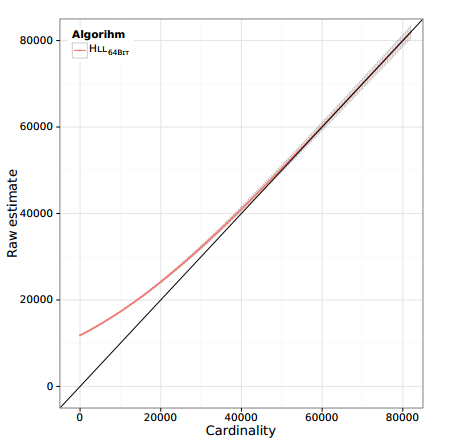
\includegraphics[scale=0.45]{img1.png}
\caption{Trung bình độ lêch thô của thuật toán $HLL_{64BIT}$}
\end{figure}
Nếu  $n > 5m$ điều chỉnh không còn đáng kể.
\end{frame}

\begin{frame}{Hiệu chỉnh độ lêch theo kinh nghiệm}
Chúng ta có thể tính toán các quan sát độ lệch và sử dụng nó để hiệu chỉnh ước lượng thô \\ 

Để làm trong thực tế:
\bi
\item Chọn 200 lực lượng bằng nội suy điểm
\item Ghi lại trung bình ước lượng thô và độ lệch(sai số).
\item Dùng k-nearest neighbor nội suy để lấy độ lệch cho một cái ước lược thô.(k = 6).
\ei
\end{frame}
\begin{frame}{Sử dụng thuật toán}
\begin{itemize}
\item Chạy thực nghiệm 3 thuật toán với các lực lượng khác nhau và so sánh phân bố error.
\bi
\item LINEARCOUNTING, bias-corrrected raw estimate, raw estimate.
\ei
\end{itemize}
\begin{figure}[h]
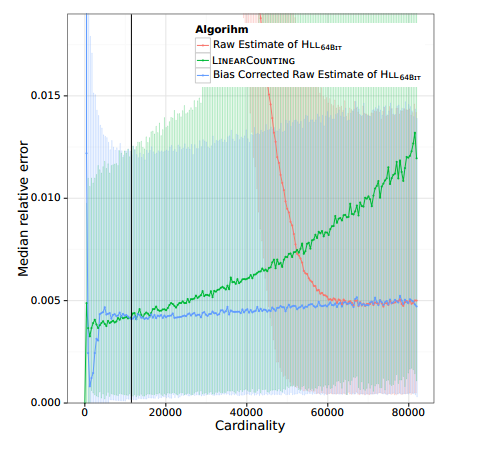
\includegraphics[scale=0.45]{img2.png}
\caption{Trung bình error của 3 thuật toán}
\end{figure}
\end{frame}
\begin{frame}{Ưu điểm của hiệu chỉnh độ lệch}
Sử dụng bias-corrected trộn với LINEARCOUNTING có ưu điểm hơn so với raw estimate trộn với LINEARCOUNTING.
\begin{itemize}
\item Lỗi cho 1 khoảng quan trọng của các lực lượng nhỏ hơn lỗi của $HLL_{64BIT}$
\item Kết quả của thuật toán không có độ lệch đáng kể.
\item Một lỗi nhỏ trong ngưỡng có kết quả nhỏ hơn về tính chính xác của kết quả thuật toán. 
\end{itemize} 
\end{frame}
\subsection{Sparse Representation}
\begin{frame}{Sparse Representation}
$Hll_NoBias $ yêu cầu bộ nhớ là 6m bit với bất kì n  \\
Trong trường hợp $n\ll m $ ta nhận thấy việc sử dụng bộ nhớ này hoàn toàn không hiệu quả \\
Vì vậy trong trường hợp này ta  phải sử dụng biểu diễn thưa(Sparse Representation) trong khi lưu cắp $(idx,\varrho(w)) $ \\
\end{frame}
\begin{frame}{Sparse Representation}
Chúng ta sẽ convert $(idx,\varrho(w)) $ ra một số nguyên bằng các biểu điễn thành một dãy bit trong đó idx là những bit cao và $\varrho(w) $ được lưu ở nhưng bit thấp. \\
Ta sẽ có một danh sách các $(idx,\varrho(w)) $ :
Để tăng tốc độ ta sử dụng một tập tạm thời tập này sẽ trộn với danh sách ở một thời điểm nào đó(vd : 25 $\%$ của danh sách) .\\
Một phần tử mới khi đưa vào  tập tạm thời nếu có phần tử cùng idx mà có giá trị lớn hơn nó trong tập rồi nó sẽ không được thêm vào .\\
Vì các tập đã được sắp xếp theo idx nên khi trộn set với list ta chỉ cần lướt một lần.

\end{frame}
\begin{frame}{Lợi ích }
\begin{itemize}
\item Giảm không gian nhớ
\item Tăng một chút thời gian chạy với việc sử dụng tập tạm thời
\end{itemize}
\end{frame}
\begin{frame}{Higher Precision for the Sparse Representa-
tion} 

Trong biểu diễn thưa ta có thể chon p' >p (Precision) nó giúp ta tăng độ  độ chính xác của thuật toán lên.\\

Điều gì xảy ra nếu khi tăng độ chính xác làm không gian lưu trữ vượt quá lên ngưỡng 6m bit.\\
Ta có thể một biểu diễn thưa với p' -> biểu điễn p bới thuật toán sau:

\end{frame}
\begin{frame}{Thuật toán chuyển độ chính xác}
Xét một cặp $(idx',\varrho(w)') $ với p' ta cần chuyển về $(idx,\varrho(w)) $ với p : 
\begin{figure}[H]
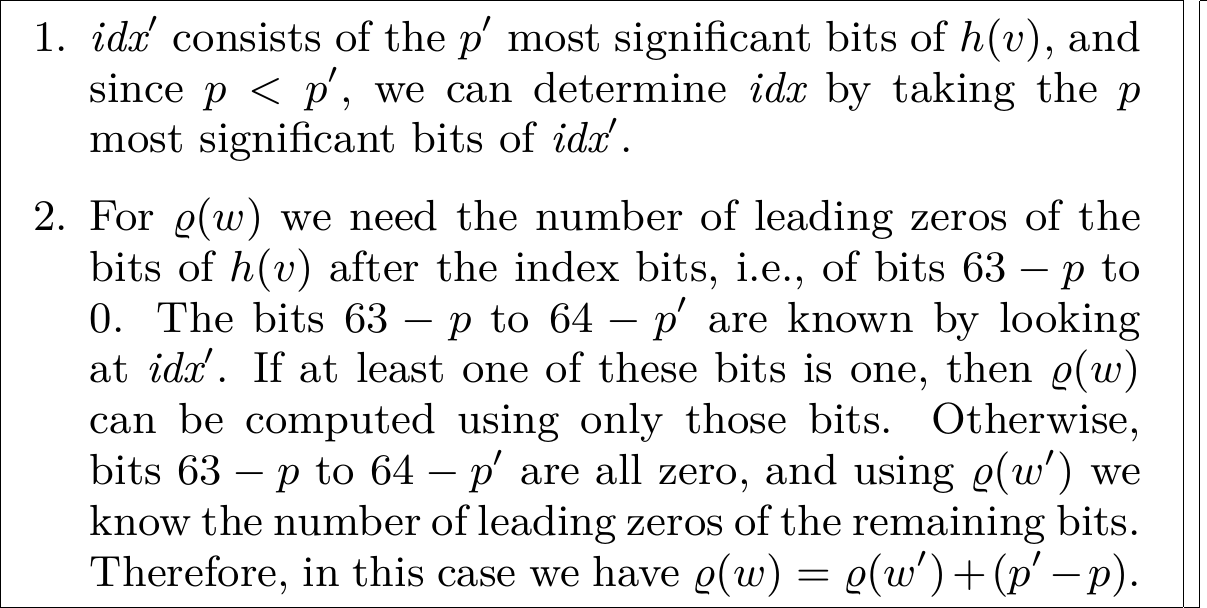
\includegraphics[scale=0.2]{HSR.png}
\caption Thuật toán chuyển Precision
\end{figure}

\end{frame}
\begin{frame}{Giảm không gian nhớ với nén thưa }
Sử dụng biểu diễn nguyên cho $(idx,\varrho(w)) $ hoạt đông tốt nhưng một phần bit của bộ nhớ vẫn bị bỏ lãng phí.
Tuy nhiên ta có thể lưu ý 2 điều sau để dữ liệu lưu được đặc khít hơn :
\begin{itemize}
\item Sử dụng số nguyên với độ rộng cứng có thể gây lãng phí.
\item Danh sách được sắp xếp ta có thể lợi dụng điều này.
\end{itemize}
\end{frame}
\begin{frame}{Thực hiện}
\begin{itemize}
\item Chúng ta sẽ encode the độ dài của biến
\item Ngoài ra chúng ta không lưu $a_1,a_2,a_3,...$ mà lưu $ a_1,a_2-a_1,a_3-a_2,...$
\end{itemize}
\end{frame}
\begin{frame}{Nhược điểm }
Khi nhìn vào việc thêm một phần tử vào danh sách nén ta sẽ thấy việc này khá là khó khăn nhưng xét trong một tiến trình trộn giữa tập tạm thời và danh sách nén thì việc này vẫn được thực hiện một cánh tuần tự.
\end{frame}
\begin{frame}{Encoding Hash Values}
Nhận thấy số lượng biến băm có thể lưu bằng biểu diễn thưa là nhỏ khi so ngưỡng chuyển từ Linear couting to bias-corrected raw
estimate . \\
Linear couting  chỉ yêu cầu m và số lượng các idex tai đấy có giá trị nhớ bằng 0.\\
Với các giá trị chuyển từ biểu diễn thưa lên biểu diễn thường $\varrho(w)$ chỉ cần lưu lại khi các bit $<x_{63-p} ,...,x_{64-p}>$ tất cả là 0. Một hàm băm tốt thì xác suất lưu lại  $\varrho(w)$ $ 2^{p-p'}$
\\Thực hiện : sử dụng 1 bit đẻ cho biết ta có lưu lại $\varrho(w)$ không 
if $<x_{63-p} ,...,x_{64-p}>$ tất cả là 0 encode :  $<x_{63-p} ,...,x_{64-p}> || <\varrho(w)>||<1>$
else $<x_{63-p} ,...,x_{64-p}> ||<0>$ 
\end{frame}
\begin{frame}{Hiệu quả không gian}
\begin{figure}[H]
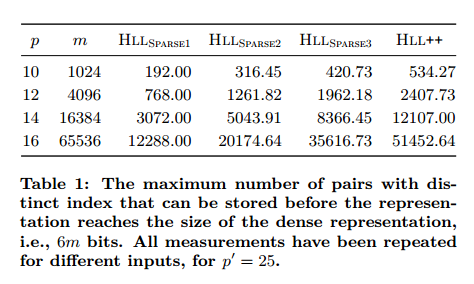
\includegraphics[scale=0.5]{img3.png}
\end{figure}
\begin{itemize}
\item $p = 14$ lưu mỗi phần tử trong biểu diễn thưa như 1 số nguyên sẽ cần 32 bit
\item Mã hóa thì điều này giảm 
\begin{itemize}
\item Độ dài trung bình 19.49 bits/phần tử
\end{itemize}
\end{itemize}
\end{frame}

\section*{Tài liệu tham khảo}

% TODO: Book
\begin{frame}{Sách tham khảo}
    \vspace{20pt}

    \bi
        \item {\color{hilight}Competitive Programming} by Steven Halim
        \item[] (Sử dụng bản 2 hoặc bản 3)
        \vspace{10pt}
        \item {\color{hilight}Bài giảng Chuyên đề} by Lê Minh Hoàng
    \ei
\end{frame}

% TODO: Overview
\begin{frame}{Các bài giảng}
 
\end{frame}
% TODO: What kind of problems we're dealing with: description/input/output



\end{document}
